\documentclass{standalone}
\usepackage{tikz}
\usetikzlibrary{spy}

\begin{document}
\begin{tikzpicture}[spy using outlines={red, rectangle,
         magnification=2, size=120, connect spies}]
     \node {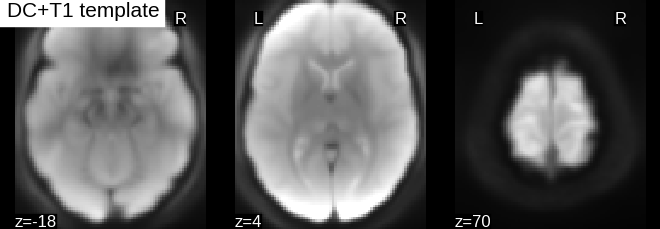
\includegraphics[width=2\linewidth]{figures/DC+T1_mean.png}};
     \spy on (-5.5,-2.5) in node at (-8,1);
     \spy on (0.,-1.5) in node at (0,2);
     \spy on (9.,-1.4) in node at (10,2);
   \end{tikzpicture}
   \begin{tikzpicture}[spy using outlines={red, rectangle,
         magnification=2, size=120, connect spies}]
     \node
         {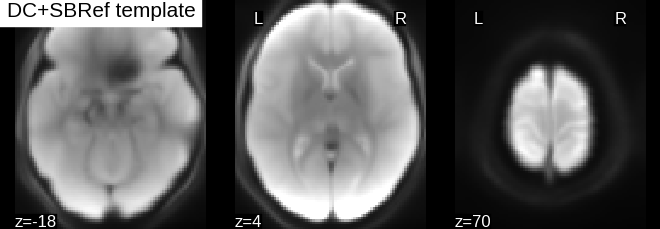
\includegraphics[width=2\linewidth]{figures/DC+SBRef_mean.png}};
     \spy on (-5.5,-2.5) in node at (-8,1);
     \spy on (0.,-1.5) in node at (0,2);
     \spy on (9,-1.4) in node at (10,2);
   \end{tikzpicture}
\end{document}
